% IWME-PRIME-01: Phase 0-3 report. Build: latexmk -pdf IWME_Phase0-3.tex
% Every number in this document is produced by `PYTHONPATH=src python -m kgirl.iwme verify`
% (kgirl repository, package src/kgirl/iwme); Appendix A is generated by that command.
\documentclass[11pt]{article}
\usepackage[letterpaper,margin=1in]{geometry}
\usepackage[T1]{fontenc}
\usepackage[utf8]{inputenc}
\usepackage[sc]{mathpazo}
\usepackage[scaled=0.88]{helvet}
\renewcommand{\ttdefault}{txtt}
\linespread{1.06}
\usepackage{amsmath,amssymb,amsthm,mathtools,bm}
\usepackage[final]{microtype}
\usepackage{booktabs,longtable,tabularx,array}
\usepackage{graphicx}
\usepackage[dvipsnames]{xcolor}
\usepackage{enumitem}
\usepackage[font=small,labelfont=bf,margin=0.5em]{caption}
\usepackage{fancyhdr}
\usepackage{newunicodechar}
\usepackage[colorlinks=true,linkcolor={[HTML]{1C5CAB}},citecolor={[HTML]{1C5CAB}},urlcolor={[HTML]{1C5CAB}}]{hyperref}
\usepackage[capitalise,noabbrev]{cleveref}

\definecolor{ink2}{HTML}{52514E}
\setlist{itemsep=2pt,topsep=3pt}
\setlength{\LTpre}{4pt}\setlength{\LTpost}{4pt}

\pagestyle{fancy}\fancyhf{}
\renewcommand{\headrulewidth}{0.3pt}
\fancyhead[L]{\small\color{ink2}IWME-PRIME-01 \textperiodcentered{} Phase 0--3 report}
\fancyhead[R]{\small\color{ink2}16 October 2026}
\fancyfoot[C]{\small\thepage}

\newtheorem{proposition}{Proposition}
\newtheorem{lemma}[proposition]{Lemma}
\newtheorem{corollary}[proposition]{Corollary}
\theoremstyle{definition}
\newtheorem{definition}{Definition}
\theoremstyle{remark}
\newtheorem*{remark}{Remark}

\newcommand{\R}{\mathbb{R}}
\newcommand{\E}{\mathbb{E}}
\newcommand{\Cov}{\operatorname{Cov}}
\newcommand{\Var}{\operatorname{Var}}
\newcommand{\Scal}{\operatorname{Scal}}
\newcommand{\rank}{\operatorname{rank}}
\newcommand{\artanh}{\operatorname{artanh}}
\newcommand{\sech}{\operatorname{sech}}
\newcommand{\softmax}{\operatorname{softmax}}
\newcommand{\Lip}{\operatorname{Lip}}
\newcommand{\lvl}[1]{\textsc{l}#1}
\newcommand{\code}[1]{\texttt{#1}}
\newcommand{\V}[1]{\hyperref[app:verify]{\textsf{#1}}}
\makeatletter\newcommand{\verifyrows}{\@@input verification_table.tex }
% Audit findings carry their own identifiers (F1, F3--F4, ...): bold identifier, then the bracket remainder.
\def\finding@split#1,#2\@nil{\textbf{#1}\if\relax\detokenize{#2}\relax\else\ (\ignorespaces\finding@strip#2\@nil)\fi}
\def\finding@strip#1,\@nil{#1}
\newenvironment{finding}[1][]{\par\smallskip\noindent\finding@split#1,\@nil.\enspace\ignorespaces}{\par\smallskip}
\makeatother

% Unicode characters used by the generated verification table (Appendix A)
\newunicodechar{±}{\ensuremath{\pm}}
\newunicodechar{²}{\ensuremath{^{2}}}
\newunicodechar{¹}{\ensuremath{^{1}}}
\newunicodechar{½}{\ensuremath{\tfrac12}}
\newunicodechar{×}{\ensuremath{\times}}
\newunicodechar{Γ}{\ensuremath{\Gamma}}
\newunicodechar{Δ}{\ensuremath{\Delta}}
\newunicodechar{Σ}{\ensuremath{\Sigma}}
\newunicodechar{α}{\ensuremath{\alpha}}
\newunicodechar{β}{\ensuremath{\beta}}
\newunicodechar{γ}{\ensuremath{\gamma}}
\newunicodechar{θ}{\ensuremath{\theta}}
\newunicodechar{κ}{\ensuremath{\kappa}}
\newunicodechar{λ}{\ensuremath{\lambda}}
\newunicodechar{μ}{\ensuremath{\mu}}
\newunicodechar{ξ}{\ensuremath{\xi}}
\newunicodechar{π}{\ensuremath{\pi}}
\newunicodechar{ρ}{\ensuremath{\rho}}
\newunicodechar{σ}{\ensuremath{\sigma}}
\newunicodechar{τ}{\ensuremath{\tau}}
\newunicodechar{φ}{\ensuremath{\varphi}}
\newunicodechar{χ}{\ensuremath{\chi}}
\newunicodechar{ψ}{\ensuremath{\psi}}
\newunicodechar{ω}{\ensuremath{\omega}}
\newunicodechar{ᵀ}{\ensuremath{^{\mathsf T}}}
\newunicodechar{‖}{\ensuremath{\Vert}}
\newunicodechar{′}{\ensuremath{'}}
\newunicodechar{″}{\ensuremath{''}}
\newunicodechar{⁺}{\ensuremath{^{+}}}
\newunicodechar{ⁿ}{\ensuremath{^{n}}}
\newunicodechar{₀}{\ensuremath{_{0}}}
\newunicodechar{₂}{\ensuremath{_{2}}}
\newunicodechar{→}{\ensuremath{\to}}
\newunicodechar{∂}{\ensuremath{\partial}}
\newunicodechar{∇}{\ensuremath{\nabla}}
\newunicodechar{∈}{\ensuremath{\in}}
\newunicodechar{−}{\ensuremath{-}}
\newunicodechar{√}{\ensuremath{\surd}}
\newunicodechar{∝}{\ensuremath{\propto}}
\newunicodechar{∞}{\ensuremath{\infty}}
\newunicodechar{∫}{\ensuremath{\textstyle\int}}
\newunicodechar{≈}{\ensuremath{\approx}}
\newunicodechar{≠}{\ensuremath{\neq}}
\newunicodechar{≤}{\ensuremath{\leq}}

\title{\textbf{Intra-dimensional Working Memory Emission}\\[3pt]
\large Intake, source-grounded audit, and formal rehabilitation of IWME Draft~1.0\\[2pt]
\normalsize IWME-PRIME-01, Phases 0--3}
\author{Investigator: K1ll\\[2pt]
\small Analysis and code: Claude (Anthropic), Opus~5.5\\
\small Phase 0--2 audit text from an earlier session (recorded as Fable~5)\\
\small Code and data: \href{https://github.com/9x25dillon/kgirl}{\code{9x25dillon/kgirl}}, package \code{src/kgirl/iwme},\\
\small branch \code{claude/iwme-phase3}}
\date{16 October 2026 \quad\textperiodcentered\quad Authorship and venue: open (Checkpoint Q6)}

\begin{document}
\maketitle
\thispagestyle{fancy}

\begin{abstract}
\noindent IWME Draft~1.0 proposes that attention-mediated working memory can shape the evolution of a physical system and of the geometry an observer measures. This report preserves the draft, reconstructs its definitions and equations, audits them against the four supplied sources, applies two corrections the investigator made to the earlier audit, and rebuilds the core as a testable model. Every numerical statement here is computed by a 47-check registry in the \code{kgirl} repository; all checks pass. Five results carry the report. (i)~The draft's four-equation system conflates observation with actuation and leaves its loop open; a repaired controlled state-space core separates them, and an observational-equivalence proposition shows that no statistic of the observables distinguishes relational memory from unmodeled physical state. (ii)~In the attention--memory architecture, retention is set by the write rate alone for a fixed attention sequence; once the attention scores read the memory, the closed-loop Jacobian $(1-\rho)I+(\rho/T)\Cov_a(v,k)$ makes retention depend on the attention temperature $T$, with a pitchfork at $T_c=1$, algebraic critical slowing $H_t\simeq(3/2\rho t)^{1/2}$, hysteresis of area $\propto(1-T)^2$, and flip or Neimark--Sacker crossings when the key--value geometry is anti-aligned or rotational. (iii)~The Inverse Resonant Toroid of \emph{The Geometry of Observation} is a parametrized 3-manifold in $\R^4$ whose Jacobian has rank three away from explicitly located circles; its published metric is wrong in three components, including a nonzero mixed term $g_{\varphi\psi}$, and its scalar curvature takes both signs, which refutes the published claim of negative curvature. (iv)~The wake-field system of the Emergent Fractal Law source contains a false defect identity, a coherence equation that leaves $[0,1]$, a Lagrangian that generates a different field equation, and a first-order time scheme whose stability limit shrinks with damping. (v)~An exact persistence-after-decoupling criterion is zero when memory cannot act on the physics, positive when it can, and separates an exponentially forgetting memory from an accumulator by its lag profile. Together they locate where evidence that memory acts on matter could come from; the report itself contains no such evidence.
\end{abstract}

\clearpage
\tableofcontents

%=====================================================================
\section{Scope, status, and how to reproduce}
%=====================================================================

\paragraph{Object.} IWME Draft~1.0 (Source~A) is preserved verbatim as an archival object; nothing below rewrites it. This report has three layers: the Phase~0--2 audit (intake, reconstruction, adversarial audit), restated with the investigator's two corrections; audits of Sources~B, C and D, which were unavailable when the Phase~0--2 report was written and have now been supplied; and Phase~3, the formal rehabilitation of the core architecture authorized by the investigator.

\paragraph{Investigator input applied.}
\begin{enumerate}[label=(\alph*)]
\item \emph{Correction to Proposition P2.} The attention-independence of forgetting holds for the exponential moving average with inputs fixed in advance. When attention scores depend on memory, the system is a closed-loop nonlinear recurrence and attention changes the sensitivity of future memory to past memory; Proposition~P3 already exhibits this. Applied as \cref{prop:P2,prop:P2prime}.
\item \emph{Correction to Finding F24.} The IRT has three parameters $(\theta,\varphi,\psi)$ embedded in four coordinates $(x,y,z,w)$ with $w=-\int_0^\psi\kappa$. Such an embedding can have a Jacobian of rank three, and wherever it does, the induced three-dimensional metric is nondegenerate; what needs repair is the published metric, which must be recomputed with its nonzero mixed components. Applied in \cref{sec:irt}, which does the recomputation before anything else in this report uses the IRT.
\item \emph{Clarification of the hypothesis.} The temperature-controlled bifurcation of the illustrative attention model is an established type of bifurcation; the investigator adopts it as a rigorous mechanism to build on, without claiming a new physical law. Recorded in \cref{sec:hypothesis}.
\end{enumerate}

\paragraph{Evidence levels.} Each claim carries a level: \lvl{0} established mathematics or engineering; \lvl{1} reasonable extrapolation; \lvl{2} hypothesis requiring experiment; \lvl{3} speculative. Every proposition proved here is \lvl{0}. Every physical reading of IWME remains \lvl{2} or \lvl{3}.

\paragraph{Reproduction.} From the root of a \code{kgirl} checkout on branch \code{claude/iwme-phase3}:
\begin{itemize}[leftmargin=1.4em]
\item \code{PYTHONPATH=src python -m kgirl.iwme verify} runs the 47 checks in about 20\,s (options \code{-{}-fast}, \code{-{}-json}, \code{-{}-latex FILE}, \code{-{}-only V22 V26});
\item \code{python -m unittest discover -s tests/iwme -t .} runs the 70 unit tests;
\item \code{PYTHONPATH=src python -m kgirl.iwme plot -o research/iwme/figures} regenerates the five figures.
\end{itemize}
Check identifiers \V{V01}--\V{V47} in the text point to Appendix~\ref{app:verify}. All variates come from the repository's deterministic logistic-map generator (\code{kgirl.evolve.chaos.ChaosRNG}); no pseudo-random generator is used anywhere.

%=====================================================================
\section{Phase 0: intake and provenance}
%=====================================================================

Five documents enter this report (\cref{tab:sources}). Sources~B--D are unpublished or non-peer-reviewed manuscripts and are cited as such. The attribution of Source~C to the ``Neurotronic Phase Caster Research Collective'' is taken from its title page.

\begin{table}[ht]
\centering\small
\caption{Sources. ``Used by Draft~1.0'' lists what the draft takes from each source; ``Audited'' says where this report checks it.}
\label{tab:sources}
\begin{tabularx}{\textwidth}{@{}l>{\raggedright\arraybackslash}X>{\raggedright\arraybackslash}X>{\raggedright\arraybackslash}p{2.6cm}@{}}
\toprule
Source & Document & Used by Draft 1.0 & Audited \\
\midrule
A & IWME Foundational Draft 1.0 & --- & \S\S3--4 \\
B & \emph{The Emergent Fractal Law and the $3^{627}$ Framework} (anonymous, 21 Oct 2025, 8 pp.) & the wake equation (draft \S6) & \S5.2 \\
C & \emph{Geometry as Emergent Uni-telligence} / \emph{The Geometry of Observation} (Neurotronic Phase Caster Research Collective, 7 Nov 2025, 19 pp.) & the history coordinate $w(\psi)$ & \S5.1 \\
D & \emph{The Convergence Point} (J.\ Edwards, with D.\ J.\ McConnell; 14 pp.) & named in the preamble, abstract and references & \S5.3 \\
E & \emph{From Triangle to Form} (M.\ Oo et al., 2026; 25 pp.) & nothing & scope note, \S5.4 \\
\bottomrule
\end{tabularx}
\end{table}

%=====================================================================
\section{Phase 1: reconstruction inventory}
%=====================================================================

\paragraph{Definitions.} D1, relational information state $H_t\in\mathcal H$ (no topology, dimension or probability structure given). D2, temporally relative environment $E_t$ with local clock $\tau_E$ (the clock is never used again; $E_t$ is said to contain physical state variables, which overlaps with $X_t$). D3, dimensional perspective $\Pi_{E,\lambda}:\mathcal H\to\mathcal O_{E,\lambda}$, an observation map. D4, working memory emission $G_{t+1}=T_{E_t,\lambda}(X_{t+1},H_{t+1},A_t)$. D5, operational presence (verbal; operationalized only as $R$ in draft \S7.2). ``Intra-dimensional'' and ``emission'' are never defined.

\paragraph{Equations} (labels assigned here). E1 $X_{t+1}=F(X_t,U_t,N_t)$; E2a--d the boxed four-equation system; E3 softmax attention without temperature; E4 the EMA memory $H_{t+1}=(1-\rho)H_t+\rho\sum_i a_{i,t}V(y_{i,t})$; E5 the additive coupling $X_{t+1}=f_E(\cdot)+B_E\Pi_E(H_t)$; E6 the grammar tuple $\mathcal L_{\mathrm{IWME}}=(\Sigma,G,\mu,\mathcal A,\mathcal M,\mathcal T)$; E7--E9 $H_\epsilon$, $D_1$, $D_q$; E10--E11 the dyadic cascade and $H_n=n\,h_2(p)$; E12 the cross-environment invariant $I(G_{E_1})\approx I(G_{E_2})$; E13--E14 the IRT coordinate $w(\psi)$ and $X_{t+1}=F_E(\dots,w_t)$; E15 the wake equation; E16 its memory-extended form with $\eta P_E(H_t,A_t)$; E17 the cycle chain $Y_t\to A_t\to H_{t+1}\to X_{t+1}\to G_{t+1}$; E18 the presence measure $R$ (a conditional mutual information); E19 the model comparison $M_0$, $M_1$, $\Delta_{\mathrm{IWME}}$.

\paragraph{Experiments.} X1 attention-controlled pattern formation; X2 relational history reconstruction; X3 cross-environment translation; X4 scale-dependent entropic grammar. None carries a full pre-registration (governing equations, units, boundary data, data source, budget, randomization, outcomes, inference plan, effect sizes, falsification thresholds, artifacts).

%=====================================================================
\section{Phase 2: audit of Draft 1.0}\label{sec:audit}
%=====================================================================

Severity: \textsc{critical} (prevents a coherent formal theory), \textsc{major} (invalidates a stated claim or test design), \textsc{minor} (notation or wording). Reviewer perspectives: [M] mathematics, [P] physics, [C] computation, [S] statistics, [R] adversarial reviewer, [E] editor.

\subsection{Architecture}

\begin{finding}[F1, critical, M/P] The observation map and the physical coupling share one symbol. D3 defines $\Pi_{E,\lambda}$ as the observer's representation of memory (hypothesis H1 of draft \S7); E2c and E5 feed $\Pi_E H_t$ into the physical dynamics (hypothesis H2). The draft insists these differ and its equations merge them. Repair: an actuation map $C_E:\mathcal H\to\mathcal U_E$ distinct from $\Pi_{E,\lambda}$; H1 is the sub-hypothesis $C_E\equiv0$.
\end{finding}

\begin{finding}[F2, critical, M] The recursive cycle is asserted and never written. $Y_t$ is a free exogenous input, so $H_t$ filters an external signal and the loop is open. Repair: $Y_t=\mathcal Y_E(X_t,Y^{\mathrm{ext}}_t,N^y_t)$.
\end{finding}

\begin{finding}[F3--F4, major] The geometric output is defined three ways (D4, E2d, \S5), and E2c and E17 disagree on whether $X_{t+1}$ reads $H_t$ or $H_{t+1}$. A physical observable can depend on $H$ only through $X$; an output that reads $H$ directly is a representation. Repair: $G^{\mathrm{phys}}_{t,\lambda}=T_{E,\lambda}(X_t)$ and $G^{\mathrm{rep}}_{t,\lambda}=T'_{E,\lambda}(X_t,H_t)$, one causal order (\cref{sec:core}).
\end{finding}

\begin{finding}[F5, major, M/S] No probability structure. Mutual information (draft \S7.2) and likelihood (\S9) need one. The minimal formalism is a controlled Markov kernel on $Z_t=(X_t,H_t)$ with emission kernels for $Y_t$ and $G_t$, a controlled POMDP.
\end{finding}

\begin{finding}[F6--F8, major/minor, E/P] ``Intra-dimensional'' is undefined; a candidate reading (within one representational perspective $\Pi_{E,\lambda}$, with no additional physical dimensions) awaits confirmation (Q1). Symbol collisions: $\lambda$ is both scale and damping (damping becomes $\gamma$ here), $H$ is both memory and entropy (entropy becomes $\mathrm H[\cdot]$), $M$ is both operator and model. $E_t$ should hold slow parameters and boundary data only; $\tau_E$ needs a concrete map or removal.
\end{finding}

\subsection{Attention and memory}\label{sec:audit-attention}

\begin{finding}[F9, major, M/R; amended per correction (a)] E4 is a first-order IIR filter whose input is a convex combination of values. \emph{For an attention sequence fixed in advance}, retention has time constant $\tau_{\mathrm{mem}}=-1/\ln(1-\rho)$ set by $\rho$ alone and attention selects content only (\cref{prop:P2}). \emph{When the scores read the memory}, as in any architecture where $q=q(H_t)$, the map is a closed-loop recurrence whose Jacobian contains $(\rho/T)\Cov_a(v,k)$, and attention changes retention (\cref{prop:P2prime}): at $T=1.2$, $\rho=0.5$, the sensitivity of $H_{10}$ to $H_0$ is $0.365$ in closed loop against $(1-\rho)^{10}=9.8\times10^{-4}$ in open loop (\V{V02}). The earlier conclusion that attention only selects content therefore holds for the fixed-input filter and fails for the feedback system. A forget gate $\rho_t=\rho(A_t)$ remains the way to make retention attention-dependent in open loop (\V{V14}).
\end{finding}

\begin{finding}[F10, major] E3 has no temperature and no score function. Ablation needs a continuous control: $s_{i,t}=\langle q(H_t),k(y_{i,t})\rangle/T$, with $T\to\infty$ uniform and $T\to0$ hard selection; $q$, $k$, $V$ must be fixed before any experiment.
\end{finding}

\begin{finding}[F11--F12, constructive] Attention sharpness is a bifurcation parameter (\cref{sec:attention}). The softmax is a Gibbs distribution with energies $-s_i$, so a physical attention operator has a standard reading: Boltzmann weighting of competing modes by growth rate, gain or overlap, with saturation supplying normalization; this is pattern selection by mode competition \cite{CrossHohenberg1993}. It is the natural candidate pathway for H2, and it is ordinary physics.
\end{finding}

\subsection{Physical coupling}
\begin{finding}[F13, major, P] $B_E\Pi_E(H_t)$ must carry the units of $X$, so $B_E$ is dimensionful. A memory-dependent additive term in a conservative system does work and needs an energy source; E5 is a stateful nonlinear controller with an EMA/softmax structure. Novelty has to be located elsewhere.
\end{finding}

\subsection{Entropy as a fractal language}
\begin{finding}[F14--F16, major/minor] The grammar tuple lacks domains and mixes layers. With a finite alphabet $\Sigma$, a constraint language $G\subseteq\Sigma^*$, a measure $\mu$ on $\Sigma^{\mathbb N}$ and a symbolization $\sigma:X\to\Sigma$, the construction is symbolic dynamics with the thermodynamic formalism \cite{Ruelle1978,LindMarcus1995,Halsey1986}; with a generating partition the entropy rate equals the Kolmogorov--Sinai entropy. The worked cascade is correct once the dyadic assumption $\epsilon=2^{-n}$ is stated: $D_q=\log_2(p^q+(1-p)^q)/(1-q)$ exactly at every level. All eight hand-computed values of the Phase~0--2 table reproduce (\V{V15}), box counting on the exact level-16 measure reproduces the closed form to $2\times10^{-16}$ (\V{V16}), and $H_n=n\,h_2(p)$ holds exactly (\V{V17}). The measure is exactly self-similar, so the draft's phrase ``increasingly structured across scales'' is incorrect. The $D_q$ spectrum is a necessary condition for a shared mechanism and far from a complete invariant. This material is a baseline \cite{Mandelbrot1974,Hentschel1983,Renyi1961}.
\end{finding}

\subsection{History dependence and identifiability}
\begin{finding}[F18, critical, M/S/R] ``Future expression may depend upon relational history not completely recoverable from its immediately observed configuration'' is trivial if ``configuration'' means the measured state (every hidden-state system) and unfalsifiable if it means the complete physical state (\cref{prop:P1}). The testable form is parametric: a specific low-complexity attention--memory class predicts held-out behaviour better than hidden-state models of matched dimension and information access.
\end{finding}

\begin{finding}[F19--F21, major] $M_1$ conditions on $H_t,A_t$, which are functions of $Y_{\le t}$, while $M_0$ is denied $Y_{\le t}$; any positive $\Delta_{\mathrm{IWME}}$ is then partly an information-access artifact. Only the observable subspace of $H$ (Kalman decomposition \cite{Kalman1960}) is identifiable. The invariant of E12 must be pre-registered as invariant under a declared transformation group, with known universality classes \cite{Turing1952,CrossHohenberg1993} as the null.
\end{finding}

\subsection{The IRT history coordinate}
\begin{finding}[F22--F23, minor/major] $\kappa(s)$ is a scalar function along a path and should be called one. $w$ is an integrator: if $\kappa=\kappa(\psi)$, $w$ is a function of $\psi$ and carries no information beyond $\psi$; with $\kappa$ driven by unobserved quantities, E13 is an accumulator with a pole at $1$, against the EMA pole at $1-\rho$. The two are distinguishable after decoupling (\cref{sec:persist}).
\end{finding}

\begin{finding}[F24, corrected per (b)] The Phase~0--2 report warned that treating $w$ as an independent coordinate while defining $w=w(\psi)$ would make the induced metric degenerate. Source~C's Definition~2.1 does something different: three parameters $(\theta,\varphi,\psi)$, four ambient coordinates $(x,y,z,w)$, $w=-\int_0^\psi\kappa$. The $4\times3$ Jacobian has rank three away from explicitly located circles, so the induced metric is nondegenerate there (\cref{prop:irt-rank}, \V{V25}). The warning applies only to Source~C's Definition~5.1 read as a four-coordinate line element on a three-manifold. The actual defect is the published metric, recomputed in \cref{sec:irt}.
\end{finding}

\begin{finding}[F25, standing position] An exponentially contracting coordinate is a reparametrization and absorbs no energy; an inverse reconstruction operator that uses later data is smoothing, which is inference in time and involves no retrocausality.
\end{finding}

\subsection{Wake-field dynamics}
\begin{finding}[F26--F29, major] Nothing in E15 is physically identified; a consistent unit assignment exists once $[W]$ is fixed, and $S$ requires an explicit coarse-graining with its own scale. E16 places a discrete-time memory inside a continuous-time PDE; it needs a zero-order hold $P_E(H_t,A_t)(x)=\sum_j(H_t)_j\varphi_j(x)$ on $[t\Delta,(t+1)\Delta)$ or a continuous-time memory (implemented as \code{HybridWake}). E15 is the damped wave equation with sources; its energy identity and a second-order scheme are in \cref{sec:wake}. A nonzero inferred $\eta$ is indistinguishable from an unmodeled source unless $P_E$ has a pre-registered form.
\end{finding}

\subsection{The presence criterion}
\begin{finding}[F31, major, S/R] E18 is conditional transfer entropy \cite{Schreiber2000}, Granger causality in information form \cite{Granger1969}. It is positive under any coupling, common cause or incomplete conditioning, so it measures coupling. The strengthened criterion, persistence after decoupling, is developed and computed in \cref{sec:persist}.
\end{finding}

\subsection{Experimental program and citations}
\begin{finding}[F32--F35] The experiments lack items 4--16 of a pre-registration; X1's ``matched conventional controllers'' is undefined while the IWME model is itself a controller; X2's success criterion is met by any latent-state model; X3 and X4 lack pre-registered invariants, symbolization and scale range. The preamble and abstract cite Source~D's ``convergence conditions and attention measurements'' and the body uses none (\cref{sec:sourceD} shows Source~D supplies none usable). References 4--8 are correctly cited; the primary sources on which the claims depend are added to the bibliography.
\end{finding}

%=====================================================================
\section{Source audits}\label{sec:sources}
%=====================================================================

\subsection{Source C: the Inverse Resonant Toroid, recomputed}\label{sec:irt}

Source~C, Definition~2.1, parametrizes $\mathcal T^{\mathrm{IRT}}\subset\R^4$ by
\begin{equation}\label{eq:irt}
X(\theta,\varphi,\psi)=\bigl(\rho\cos\theta,\;\rho\sin\theta,\;r\sin\varphi\,\sinh\beta\psi,\;w(\psi)\bigr),
\end{equation}
where $\rho=u\,e^{-\alpha\psi}$, $u=R-r\cos\varphi$ and $w=-\int_0^\psi\kappa$, with $R>r>0$, $\alpha,\beta>0$, $\psi\ge0$. The computations use $(R,r,\alpha,\beta)=(3,1,0.3,0.5)$ and two kernels: the constant $\kappa\equiv1$ and the single mode of Source~C's eq.~(15), $\kappa(\psi)=e^{-0.2\psi}\cos2\psi$.

\begin{proposition}[Induced metric; \lvl{0}]\label{prop:irt-metric}
In the order $(\theta,\varphi,\psi)$, with $g_{\theta\varphi}=g_{\theta\psi}=0$,
\begin{align*}
g_{\theta\theta}&=u^2e^{-2\alpha\psi},\\
g_{\varphi\varphi}&=r^2\bigl(\sin^2\!\varphi\,e^{-2\alpha\psi}+\cos^2\!\varphi\,\sinh^2\!\beta\psi\bigr),\\
g_{\varphi\psi}&=r\sin\varphi\,\bigl(\beta r\cos\varphi\,\sinh\beta\psi\cosh\beta\psi-\alpha u\,e^{-2\alpha\psi}\bigr),\\
g_{\psi\psi}&=\alpha^2u^2e^{-2\alpha\psi}+\beta^2r^2\sin^2\!\varphi\,\cosh^2\!\beta\psi+\kappa(\psi)^2,\\
\det g&=u^2e^{-2\alpha\psi}\bigl[r^2e^{-2\alpha\psi}D^2+\kappa^2g_{\varphi\varphi}\bigr],
\end{align*}
with $D=\beta r\sin^2\!\varphi\cosh\beta\psi+\alpha u\cos\varphi\sinh\beta\psi$.
\end{proposition}
\begin{proof}
$X_\theta=\rho\,\hat e_\theta$ is orthogonal to $X_\varphi=(\rho_\varphi\hat e_\rho,\,z_\varphi,\,0)$ and $X_\psi=(\rho_\psi\hat e_\rho,\,z_\psi,\,-\kappa)$, which gives the $\theta$ row. The $(\varphi,\psi)$ block is the Gram matrix of $X_\varphi,X_\psi$; its determinant is, by Cauchy--Binet, the sum of the squared $2\times2$ minors in the frame $(\hat e_\rho,\hat e_z,\hat e_w)$: $(\rho_\varphi z_\psi-z_\varphi\rho_\psi)^2=r^2e^{-2\alpha\psi}D^2$, $(\rho_\varphi\kappa)^2$ and $(z_\varphi\kappa)^2$, and the last two sum to $\kappa^2g_{\varphi\varphi}$. A symbolic computation confirms every component and the determinant (\V{V23}); the closed form agrees with $J^{\mathsf T}J$ to $2\times10^{-15}$ (\V{V22}).
\end{proof}

\begin{proposition}[Rank; \lvl{0}]\label{prop:irt-rank}
$\rank J=3$ except on the circles (all $\theta$) where $\det g=0$:
\[
\{\psi=0,\ \sin\varphi=0\}\;\cup\;\{\kappa(\psi)=0,\ D(\varphi,\psi)=0\}.
\]
\end{proposition}
\begin{proof}
Both bracketed terms of $\det g$ are nonnegative and $u>0$. $g_{\varphi\varphi}=0$ forces $\sin\varphi=0$ and $\cos\varphi\sinh\beta\psi=0$, hence $\psi=0$, where $D=0$ as well. Otherwise $\det g=0$ needs $\kappa=0$ and $D=0$.
\end{proof}

For $\kappa\equiv1$ only the two boundary folds at $\psi=0$ remain (the $\psi=0$ slice lies in the plane $z=0$, which folds the $\varphi$-circle). For $\kappa=e^{-0.2\psi}\cos2\psi$ there are two further circles on each zero $\psi_k=(2k+1)\pi/4$ of $\kappa$; on $(0,6]$ these are at $\varphi\approx(2.3049,3.9783)$, $(2.0483,4.2349)$, $(2.0025,4.2807)$, $(1.9932,4.2900)$. The numerical rank is 2 and $\det g<10^{-28}$ on all of them and 3 at generic points (\V{V25}). This confirms correction (b).

\paragraph{The published metric.} Source~C's Appendix~A.1 prints $g_{\varphi\varphi}=r^2e^{-2\alpha\psi}\cosh^2\!\beta\psi$, a $\sinh^2$ in place of $\cosh^2$ in $g_{\psi\psi}$, and $g_{\varphi\psi}=0$. The $g_{\psi\psi}$ error has the closed form $g_{\psi\psi}^{\mathrm{true}}-g_{\psi\psi}^{\mathrm{A.1}}=\beta^2r^2\sin^2\!\varphi$. At $(\varphi,\psi)=(2.5,1.7)$ the relative errors are $3.6\%$ in $g_{\varphi\varphi}$ and $8.0\%$ in $g_{\psi\psi}$, and the omitted mixed component is $g_{\varphi\psi}=-0.563$ (\V{V24}); $g_{\theta\theta}$ and the vanishing $\theta$-row are right.

\paragraph{Christoffel symbols.} With the non-diagonal block, $\Gamma^a_{ij}=g^{ab}\Gamma_{b,ij}$ for $a,b\in\{\varphi,\psi\}$ and $\Gamma_{b,ij}=\tfrac12(\partial_ig_{jb}+\partial_jg_{ib}-\partial_bg_{ij})$; in the $\theta$ row, $\Gamma^\theta_{\theta\varphi}=r\sin\varphi/u$ and $\Gamma^\theta_{\theta\psi}=-\alpha$. Source~C's eq.~(28) gets $\Gamma^\theta_{\theta\psi}$ right and omits $\Gamma^\theta_{\theta\varphi}$. Its other entries fail even against its own diagonal metric: the printed $\Gamma^\psi_{\theta\theta}=-\alpha u^2e^{-2\alpha\psi}/g_{\psi\psi}$ has the wrong sign ($-1.278$ printed, $+1.278$ from eq.~(27), at $(\varphi,\psi)=(0.9,1.2)$), and the printed $\Gamma^\psi_{\varphi\varphi}$ is $+0.358$ against $+0.033$ (\V{V31}). The values from the correct metric at that point are $\Gamma^\psi_{\theta\theta}=+0.831$, $\Gamma^\psi_{\varphi\varphi}=-0.562$, $\Gamma^\varphi_{\varphi\psi}=+0.189$ (printed $-0.031$).

\begin{proposition}[Scalar curvature; \lvl{0}]\label{prop:irt-curv}
Let $\Sigma$ be the profile surface $(\varphi,\psi)\mapsto(\rho,z,w)\in\R^3$ with metric $g_\Sigma$ (the $(\varphi,\psi)$ block). Then $M$ is the warped product $\Sigma\times_\rho S^1$ and
\[
\Scal=2K_\Sigma-2\,\frac{\Delta_\Sigma\rho}{\rho},\qquad K_\Sigma=\frac{\det\mathrm{II}_\Sigma}{\det g_\Sigma}.
\]
$\Scal$ depends on $\kappa$ only through $\kappa$ and $\kappa'$.
\end{proposition}
\begin{proof}
$g=g_\Sigma+\rho^2d\theta^2$, and for a warped product with a one-dimensional flat fibre $\Scal=\Scal_\Sigma-2\Delta_\Sigma\rho/\rho$ \cite{ONeill1983}. For the second claim, $M$ is a hypersurface of flat $\R^4$, so the Gauss equation gives $\Scal=(\operatorname{tr}S)^2-\operatorname{tr}S^2$ with $S=g^{-1}\mathrm{II}$ \cite{doCarmo1992}; $\mathrm{II}$ involves $X$ and its second derivatives, and $X_{\psi\psi}$ carries $-\kappa'$ and no higher derivative.
\end{proof}

Three independent numerical routes, the Gauss equation with exact derivatives, the intrinsic Riemann tensor from finite differences of the metric, and the warped-product formula, agree to $3\times10^{-6}$ (relative) at ten test points (\V{V26}). Changing $\kappa''(\psi_0)$ from $0$ to $14$ with $\kappa(\psi_0),\kappa'(\psi_0)$ fixed leaves $\Scal(\psi_0)$ unchanged to $2\times10^{-8}$ (\V{V27}).

\begin{proposition}[Sign; \lvl{0}]\label{prop:irt-sign}
For constant $\kappa\equiv\kappa_0$, $\Scal\to2K_{T_\psi}$ as $\kappa_0\to\infty$, where $T_\psi$ is the slice $\psi=\mathrm{const}$, a torus of revolution with elliptical profile and
\[
K_{T_\psi}(\varphi)=-\frac{r^3\sinh^2\!\beta\psi\,\cos\varphi}{u\,g_{\varphi\varphi}^2}.
\]
Hence $\Scal$ takes both signs for all large $\kappa_0$; $\int_{T_\psi}K\,dA=0$ by Gauss--Bonnet on every slice with $\psi>0$.
\end{proposition}
Numerically the error $\lvert\Scal-2K_{T_\psi}\rvert/\lvert2K_{T_\psi}\rvert$ is $1.6\times10^{-1}$, $1.6\times10^{-3}$, $1.6\times10^{-5}$ at $\kappa_0=10,100,1000$, consistent with $O(\kappa_0^{-2})$, and $K_{T_\psi}<0$ exactly where $\cos\varphi>0$ (\V{V28}). At $\kappa_0=1$ the curvature is negative on $67\%$ and positive on $33\%$ of the chart $(\varphi,\psi)\in[0,2\pi)\times[0.05,4]$; for the damped kernel the split is $56\%/44\%$ (\V{V29}, \cref{fig:irt}). Source~C's conclusion ``negative curvature confirms inward-focusing geometry'' is false, and its eq.~(29) disagrees with the curvature in value and in sign (sign differs at 2 of 5 test points; e.g.\ $+2.736$ against $-8.186$, \V{V30}); it also contains $\kappa''/\kappa$, which \cref{prop:irt-curv} excludes, and $3\beta^2/\cosh^2\!\beta\psi$, which lacks the inverse-length-squared units of a scalar curvature.

\begin{figure}[t]
\centering
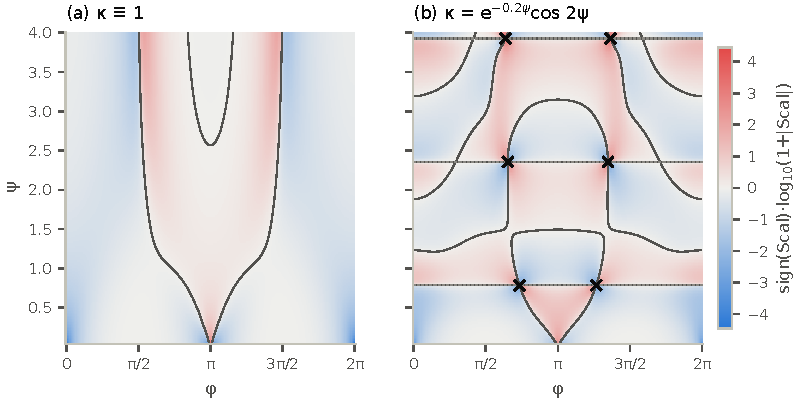
\includegraphics[width=\textwidth]{figures/fig_irt.pdf}
\caption{Scalar curvature of the IRT over the chart, signed logarithmic scale (blue negative, red positive, dark contour $\Scal=0$). (a) $\kappa\equiv1$. (b) $\kappa=e^{-0.2\psi}\cos2\psi$; dotted lines mark the zeros of $\kappa$ and crosses the rank-2 circles of \cref{prop:irt-rank}. Both signs occur on sets of large measure.}
\label{fig:irt}
\end{figure}

\paragraph{Shadow reconstruction.} Source~C's eq.~(16) is offered as the integral of eq.~(15) and is incorrect: it integrates the exponential and the cosine factors separately. Its derivative misses $-\kappa$ by up to $2.92$ on $[0.1,3]$ and it gives $w(0)=-5\ne0$; the exact antiderivative $-\sum_nA_n\bigl[e^{-\lambda_n\tau}(\omega_n\sin(\omega_n\tau+\phi_n)-\lambda_n\cos(\omega_n\tau+\phi_n))/(\lambda_n^2+\omega_n^2)\bigr]_0^\psi$ is implemented (\V{V32}).

\paragraph{Definition 5.1.} Source~C also writes $ds^2=g_{\mu\nu}dx^\mu dx^\nu+h(\psi)\,dw^2$ with $h=e^{2\beta\psi}$ and $g_{\mu\nu}$ ``the standard toroidal metric''. Read on the 3-manifold, $dw=-\kappa\,d\psi$ and the line element is a third metric, with $e^{2\beta\psi}\kappa^2$ in place of $\kappa^2$; read as a metric in four coordinates on a three-manifold it is degenerate, which is the case the original F24 described. The source needs one metric. The induced metric of \cref{prop:irt-metric} is the one consistent with Definition~2.1.

\paragraph{Consequences for IWME.} The history coordinate $w$ remains an integrator (F23). If the IRT stays in the program, its geometry is that of \cref{prop:irt-metric,prop:irt-curv}; its published curvature claims, reception principle and ``higher-dimensional intelligence'' interpretation are \lvl{3} and play no role in any test below.

\subsection{Source B: the Emergent Fractal Law and the wake system}\label{sec:sourceB}

\paragraph{Categorical content.} Several statements are ill-typed as written. Axiom~1.3 asks for a profunctor $V$ ``mediating $\pi\tau\Rightarrow\tau\pi$'' with $\tau:\mathcal S\to\mathcal S_{\le m}$, $\pi:\mathcal S_{\le m}\to\mathcal S$; $\pi\tau$ is an endofunctor of $\mathcal S$ and $\tau\pi$ an endofunctor of $\mathcal S_{\le m}$, so no natural transformation between them exists. Definition~2.1 (Fubini--Stokes) has the same defect. $[\tau,\delta]\simeq0$ commutes a functor with a coboundary operator on cochains, which needs a chain-level action of $\tau$ that is never given. Theorem~1.1 cites Axioms A--D, which are numbered 1.1--1.4. The model example asserts that formality obstructions of $A_\infty$-algebras become exact at a finite stage; non-formal algebras exist (formality forces all Massey products to vanish \cite{DGMS1975}, and the complement of the Borromean rings carries a nonvanishing triple Massey product), so Axiom~1.2 fails in its own model. The effective dimension $D_{\mathrm{eff}}=\limsup\log N(r)/\log\lambda^r$ with $N(r)\sim\lambda^r$ equals $1$ identically (\V{V21}); a dimension needs the branching number and the scale factor to be independent, $D=\log b/\log\lambda$.

\paragraph{A finite model of the EFL fixed point.} The Phase~0--2 report asked for a finite-dimensional model before any higher-categorical claim. Take measures on $[0,1]$, $\Phi_\lambda$ the Hutchinson operator $(\Phi\mu)(A)=p\,\mu(2A)+(1-p)\,\mu(2A-1)$. It contracts the Wasserstein-1 distance by exactly $\tfrac12$ (the two branches do not overlap), its unique fixed point is the binomial measure, and $\Phi(\text{binomial}_n)=\text{binomial}_{n+1}$; the measured ratio is $\tfrac12$ to $2\times10^{-14}$ (\V{V20}) \cite{Hutchinson1981}. This realizes ``$E\simeq\Phi_\lambda E$'' as a theorem, with the colimit replaced by the limit of iterates.

\paragraph{The PDE system (4.2).} With damping renamed $\gamma$:
\begin{enumerate}[label=(B\arabic*)]
\item \emph{Defect identity (Prop.~4.2), false.} For a vortex of charge $m$, $\nabla\times\nabla\theta=2\pi m\,\delta$ and $\Delta\theta=\nabla\cdot\nabla\theta=0$ in distributions \cite{Mermin1979}. On a lattice, the circulation around every square loop enclosing the core is $2\pi m$ for $m\in\{1,-1,2\}$ (loops of half-width $\ge2$), and the flux of $\nabla\theta$ through each loop, the integral of $\Delta\theta$ inside it, is $0$ to machine precision; Prop.~4.2 predicts $2\pi m$ (\V{V36}). Sources for $\mathcal W$ must be built from the vorticity of the phase.
\item \emph{Coherence (4.2c).} $\partial_tc+\mu c=-\gamma_c\lvert\nabla\arg\psi\rvert^2$ has the steady state $-\gamma_c\lvert\nabla\theta\rvert^2/\mu<0$; with $c_0=1$, $\mu=1$, $\gamma_c\lvert\nabla\theta\rvert^2=0.5$ it crosses $0$ at $t=\ln3$ (\V{V37}), and near a vortex $c^*=-\gamma_cm^2/(\mu r^2)\to-\infty$. The stated range $c\in[0,1]$ is not invariant; a bounded coherence needs a nonlinear self-term such as $\mu c(1-c)$.
\item \emph{Entropy (4.2b).} $\partial_tS-D_S\Delta S=-\nabla\cdot J_S$ with $J_S=-\kappa\nabla S$ is diffusion with coefficient $D_S+\kappa$; the flux term duplicates $D_S$. Signs are consistent and the problem is well posed; with $\partial_nS=0$ the total $\int S$ is conserved and there is no production term.
\item \emph{Energy (Prop.~4.1).} The conclusion ``if $S$ and $c$ are stationary, $\mathcal E(t)$ decays'' needs zero forcing: with a stationary nonzero $\alpha\Delta S$ and the wake at rest, the energy rises from $5.6\times10^{-8}$ to $3.6\times10^{-5}$ (\V{V38}).
\item \emph{Well-posedness (Thm.~4.1).} Point sources $q_k\delta(x-x_k)$ lie outside $H^{-1}$ for $d\ge2$: the 2D static response $-\ln r/2\pi$ has $\int_{h<r<1}\lvert\nabla W\rvert^2=\ln(1/h)/2\pi\to\infty$ (\V{V42}), so the claimed $C([0,T];H^1)$ solution does not exist without regularized cores.
\item \emph{Variational principle.} The Euler--Lagrange equation of (4.4) is $W_{tt}-v^2W_{xx}+v^2\omega^2W=\chi v^2S_{xx}+v^2\xi(1-c)$: it has a restoring term absent from (4.2a), and its coherence source is $(1-c)$ where (4.2a) has $\partial_t(1-c)$ (\V{V41}).
\item \emph{Worked examples.} The localized steady wake (4.9) requires a mass term $\gamma_mW$; with (4.2a) as written the steady response to a point source grows with the domain, $W(0)=L/2$ for $L=1,2,4$ (\V{V39}). For the decoherence pulse the uniform mode reaches $W(\infty)=\beta/\gamma$ for every $\sigma$ (2.000000 at $\sigma=2$ and $0.5$); Source~B states $\beta\sigma/\gamma$ (\V{V40}).
\item \emph{Scheme (4.13).} It discretizes the damping with a backward difference: first order in time (observed order $1.005$, against $1.998$ for centered damping, \V{V34}), and stable only for $v\Delta t/\Delta x<\sqrt{(1-\gamma\Delta t/2)/d}$ with $\gamma\Delta t<2$. The centered scheme of \cref{sec:wake} is stable up to $1/\sqrt d$ whatever $\gamma\Delta t$ (\V{V33}, \cref{fig:wake}a).
\end{enumerate}

\paragraph{AI instantiation (4.10).} $\mathrm{PC}(E)=(\max_iw_i-1/M)/(1-1/M)$ with $w$ the principal eigenvector of $EE^{\mathsf T}$ scores $M$ identical answers $0$, mutually orthogonal answers $1$, and is undefined for an antipodal pair (the eigenvector changes sign and $\sum w_i=0$) (\V{V46}). \code{kgirl.main.spectral\_coherence} already replaces it, on its fallback path, by the rescaled principal share $(\lambda_{\max}/M-1/M)/(1-1/M)$, which scores agreement correctly and is sign-blind (an antipodal pair scores 1). The rescaled squared mean resultant length $(\lVert\bar e\rVert^2-1/M)/(1-1/M)$, the order parameter of unit vectors \cite{Kuramoto1984}, scores the three cases $1,0,0$ and is the sign-aware choice. \code{PhaseCoherence.scalar} in \code{kgirl.main} still applies (4.10) when its optional topological backend is present.

\subsection{Source D: The Convergence Point}\label{sec:sourceD}

Draft~1.0 cites Source~D for ``convergence conditions and attention measurements''. Source~D's attention condition is relational and qualitative, and its quantitative content is the WR-039T pipeline. The checks:
\begin{itemize}
\item \emph{Tier 1.} The reported Walsh coefficients of $[1,1,1,-1,1,1,1,1]$ are $[4,0,0,-4,0,4,4,0]$. The transform is $[6,2,2,-2,-2,2,2,-2]$ in natural order; no ordering or normalization yields the reported vector, which is the transform of $[1,1,1,-1,-1,1,1,1]$. Both vectors have energy $64=N\cdot E_{\mathrm{in}}$, so the reported Parseval PASS cannot detect the error (\V{V43}): Parseval holds for every orthogonal transform of every signal and verifies the implementation of the transform only.
\item \emph{Tier 2.} $\varphi(a^k)=\varphi(a)^k$ for $\varphi=$ reduction mod 3 on $\mathbb Z_9$ holds for all $a,k$ (0 failures in 279) because 3 divides 9; a check that cannot fail carries no information. No unital ring map $\mathbb Z_4\to\mathbb Z_3$ exists (\V{V44}). PAEF scores are reported without a formula.
\item \emph{Prediction 5.} ``Energy concentrated in low-order Walsh coefficients'' is maximal (share $1.000$) for a constant signal and $0.011$ for chaotic noise (\V{V45}): it measures smoothness, the reverse of the complexity it is meant to index.
\item \emph{Tier 8 and the appendix.} One 100-iteration run per system, $546.3\to543.5$\,ms ($-0.51\%$) with no dispersion, cannot separate system differences from serving-side variation (context length, caching, batching, sampling). The TRIBE~v2 appendix compares model-predicted cortical responses to single sentences without statistics; the audio-only versus trimodal contrast follows from which encoder sees the words.
\end{itemize}
Source~D therefore provides no attention measurement IWME can use. It can be cited for the conceptual claim that attention is a relational condition; the abstract's dependency should be removed or rephrased.

\subsection{Source E: scope note}
\emph{From Triangle to Form} (E8 holography, the proton radius) is outside IWME's dependency graph and is not audited here. One methodological point transfers: its automated checks, such as $\sqrt{12/\cos^2 30^\circ}=4$, verify arithmetic identities that hold by construction; like Source~D's Parseval check, they test the code and say nothing about the physical identifications.

%=====================================================================
\section{Phase 3: formal rehabilitation}\label{sec:phase3}
%=====================================================================

\subsection{Repaired core}\label{sec:core}
One causal order, the loop closed, observation separated from actuation:
\begin{equation}\label{eq:core}
\begin{aligned}
Y_t&=\mathcal Y_E\bigl(X_t,\,Y_t^{\mathrm{ext}},\,N^y_t\bigr), & A_t&=\mathcal A(H_t,Y_t,E_t)\in\Delta^{n-1},\\
H_{t+1}&=\mathcal M\bigl(H_t,A_t,Y_t,N^h_t\bigr), & X_{t+1}&=F_E\bigl(X_t,U_t,N^x_t,\,C_E(H_t)\bigr),\\
G^{\mathrm{phys}}_{t,\lambda}&=T_{E,\lambda}(X_t), & G^{\mathrm{rep}}_{t,\lambda}&=T'_{E,\lambda}(X_t,H_t).
\end{aligned}
\end{equation}
$E_t$ holds parameters and boundary data; $\Pi_{E,\lambda}$ enters only through $T'$; H1 is $C_E\equiv0$ and H2 is $C_E\ne0$. With the noises independent, $Z_t=(X_t,H_t)$ is a controlled Markov chain and $(Y_t,G_t)$ are its emissions (a controlled POMDP). \emph{Emission} is then the map $\mathcal M\circ(\mathcal A,\mathcal Y_E)$ together with $C_E$: what memory writes and what it sends to the physics. \emph{Intra-dimensional} remains the candidate reading of F6 until confirmed (Q1). The implementation is \code{kgirl.iwme.core.IWMECore}.

\begin{proposition}[Observational equivalence; \lvl{0}]\label{prop:P1}
The law of $(Y_t,G_t)_{t\ge0}$ given $(U_t,E_t)$ generated by \eqref{eq:core} is generated by a single-state model $Z_{t+1}=F'(Z_t,U_t,E_t,N_t)$, $Y_t=\mathcal Y'(Z_t,N^y_t)$, $G_t=T'(Z_t)$ with no distinguished memory variable.
\end{proposition}
\begin{proof}
With $Y=\mathcal Y_E(X,Y^{\mathrm{ext}},N^y)$, set
\[
F'(Z,\cdot)=\Bigl(F_E\bigl(X,U,N^x,C_E(H)\bigr),\ \mathcal M\bigl(H,\mathcal A(H,Y,E),Y,N^h\bigr)\Bigr),\qquad T'(Z)=T(X).
\]
Substitution reproduces \eqref{eq:core}. The unit test \code{test\_augmented\_state\_reproduces\_observables} checks the implementation on a nonlinear instance.
\end{proof}
No statistic of the observables separates relational memory from unmodeled physical state. Evidence for IWME can come from parametric restrictions on $(\mathcal A,\mathcal M,C_E)$ that beat matched hidden-state models, or from interventions on the memory substrate independent of $X$.

\subsection{Hypothesis}\label{sec:hypothesis}
The investigator's clarification fixes the status of the attention mechanism: the temperature-controlled bifurcation of \cref{sec:attention} is established mathematics (the mean-field pitchfork of Curie--Weiss and Hopfield type \cite{Hopfield1982}) and serves as the mechanism on which predictions are built. The working hypothesis for Phases 3--4, pending the formal answer to Q3, is the parametric one: \emph{an attention--memory model class with temperature $T$ and write rate $\rho$ predicts held-out behaviour of a physical system after interaction better than hidden-state models of matched latent dimension and identical information access $(X_{\le t},Y_{\le t},E_{\le t},U_{\le t})$} (\lvl{2}). The physical claim $C_E\ne0$ is retained as the explicitly labeled extension M4 (\lvl{2}--\lvl{3}).

\subsection{Persistence after decoupling}\label{sec:persist}
Interact $A$ and $B$ for $t<t_c$, sever the channel at $t_c$, estimate the physical state $\hat X^A_{t_c}$ as completely as the instruments allow, and define
\begin{equation}
R_{\mathrm{persist}}(\ell)=I\bigl(G^A_{t_c+\ell}\,;\,Y^B_{<t_c}\bigm\vert\hat X^A_{t_c},U,E\bigr).
\end{equation}
If the estimate were complete and the dynamics Markov, $R_{\mathrm{persist}}=0$. For the linear-Gaussian instance $H_{t+1}=\mu H_t+\rho Y^B_t$ ($\mu=1-\rho$ EMA, $\mu=1$ accumulator), $X_{t+1}=aX_t+cH_t+s_x\xi_t$, $G_t=X_t+s_g\zeta_t$, the conditional mutual information is computed exactly from covariances (\code{persistence\_information}; $a=0.8$, $\rho=0.3$, $s_x=s_g=0.1$, $t_c=40$):
\begin{itemize}
\item under H1 ($c=0$), $R_{\mathrm{persist}}=0$ exactly;
\item with $c=0.5$, the 30-step block carries $1.366$ bits given $X_{t_c}$;
\item given $(X_{t_c},H_{t_c})$ it drops to $10^{-14}$: the criterion certifies state incompleteness, as \cref{prop:P1} requires;
\item the lag profile separates memory kinds: at lag 60 the EMA memory gives $1.5\times10^{-10}$ bits and the accumulator (the pole of the IRT integrator $w$) $2.68$ bits (\V{V47}, \cref{fig:wake}b).
\end{itemize}
The parametric content of IWME enters through this profile: an EMA memory predicts geometric decay governed by $1-\rho$, and the attention model predicts how that decay changes with $T$ (\cref{sec:attention}). A pre-registration skeleton:

\begin{table}[ht]
\centering\small
\caption{Protocol B (persistence after decoupling), pre-registration skeleton.}
\label{tab:protocolB}
\begin{tabularx}{\textwidth}{@{}l>{\raggedright\arraybackslash}X@{}}
\toprule
Item & Specification \\
\midrule
Hypothesis & $R_{\mathrm{persist}}(\ell)>0$ after severing, with lag profile predicted by the attention--memory class at fitted $(T,\rho)$ better than by matched hidden-state models (\lvl{2}). \\
Arms & coupled then severed; never coupled ($C_E$ arm control); severed with maximal state measurement (incompleteness control). \\
Estimand & $R_{\mathrm{persist}}(\ell)$, $\ell=1,\dots,L$, with $\hat X_{t_c}$ covariance reported. \\
Models & M1 attention--EMA; M1$'$ attention with forget gate; M0 linear-Gaussian latent model of matched dimension; M0$'$ accumulator; all given identical inputs. \\
Outcome & held-out log-likelihood of $G_{t>t_c}$; primary contrast M1 versus best M0 at equal parameter count. \\
Falsification & M1 does not beat M0 by a pre-set margin, or the fitted lag profile is flat (accumulator-like) where M1 predicts decay. \\
Determinism & logistic-map variates (\code{ChaosRNG}), seeds listed; code \code{kgirl.iwme.core}. \\
\bottomrule
\end{tabularx}
\end{table}

\subsection{Attention theory}\label{sec:attention}
Keys $k_i$, values $v_i$, scores $s_i=\langle H+b,k_i\rangle/T$ with an input bias $b$, weights $a=\softmax(s)$, read $m(H)=\sum_ia_iv_i$, and $\Phi(H)=(1-\rho)H+\rho\,m(H)$. Let $D_k,D_v$ be the diameters of the key and value sets and $C_a(H)=\sum_ia_i(v_i-m)(k_i-\bar k)^{\mathsf T}$, $\bar k=\sum_ia_ik_i$.

\begin{proposition}[P2, open loop; \lvl{0}]\label{prop:P2}
If the read sequence $m_s$ is fixed in advance, $H_t=(1-\rho)^tH_0+\rho\sum_{s<t}(1-\rho)^{t-1-s}m_s$ and $\partial H_t/\partial H_{t-k}=(1-\rho)^kI$ for every attention sequence (\V{V01}).
\end{proposition}

\begin{proposition}[P2$'$, closed loop; \lvl{0}]\label{prop:P2prime}
\[
D\Phi(H)=(1-\rho)I+\frac{\rho}{T}\,C_a(H),\qquad \frac{\partial H_t}{\partial H_s}=\prod_{\tau=s}^{t-1}D\Phi(H_\tau)\quad\text{(ordered)}.
\]
Retention therefore depends on $T$ and on the key--value geometry.
\end{proposition}
\begin{proof}
$\partial a_i/\partial H=a_i(k_i-\bar k)/T$, so $Dm=T^{-1}\sum_iv_i a_i(k_i-\bar k)^{\mathsf T}=C_a/T$ since $\sum_ia_i(k_i-\bar k)=0$; the chain rule gives the product.
\end{proof}
At $H=0$ in the two-point example below the retention time $-1/\ln\mu(0)$ is $41.5$, $5.48$, $2.47$ steps at $T=1.05,1.5,3$ and tends to $\tau_{\mathrm{mem}}=1.443$ as $T\to\infty$ (\V{V03}); along a trajectory at $T=1.2$ the closed-loop sensitivity at lag 10 is 374 times the open-loop value (\V{V02}). \Cref{fig:retention}a shows the retention time at the stable state diverging at $T_c$ from both sides.

\begin{lemma}[Contraction; \lvl{0}]\label{lem:popoviciu}
$\lVert C_a\rVert_{\mathrm{op}}\le D_vD_k/4$ for every weight vector $a$. Hence $\Lip(\Phi)\le1-\rho+\rho D_vD_k/(4T)<1$ when $T>D_vD_k/4$, and every memory trajectory is entrained by its inputs.
\end{lemma}
\begin{proof}
For unit $x,y$, $x^{\mathsf T}C_ay=\Cov_a(\langle x,v\rangle,\langle y,k\rangle)\le\sqrt{\Var_a\langle x,v\rangle\,\Var_a\langle y,k\rangle}$, and a distribution on an interval of length $\ell$ has variance at most $\ell^2/4$ (compare with the midpoint). The projections have ranges at most $D_v$ and $D_k$.
\end{proof}
The bound is attained in the two-point example at $H=0$, where $\lVert C_a\rVert=1=D_vD_k/4$ (\V{V05}); on random configurations the worst ratio is $0.958$ (\V{V04}). This sharpens the Phase~0--2 bound $D_vD_k/T$, which gave $T>4$ for an exact threshold of $1$.

\begin{proposition}[P3, pitchfork and critical slowing; \lvl{0}]\label{prop:P3}
Take $n=2$, $d=1$, $v=k=(+1,-1)$, so $m(H)=\tanh\bigl((H+b)/T\bigr)$. At $b=0$: for $T>1$ the unique fixed point $0$ is stable with multiplier $1-\rho+\rho/T$; for $T<1$ it is unstable and $\pm H^*(T)$, $H^*=\tanh(H^*/T)$, are stable with multipliers $1-\rho+\rho(1-H^{*2})/T\in(1-\rho,1)$; $H^*\approx T\sqrt{3(1-T)}$ near $T_c=1$. At $T=1$ the fixed point is unique and attracting with
\[
H_t\simeq\Bigl(\frac{3}{2\rho t}\Bigr)^{1/2}.
\]
\end{proposition}
\begin{proof}
The fixed-point and stability statements follow from the concavity of $\tanh(\cdot/T)$ on $H>0$ and its slope at the crossing. At $T=1$, $\Phi(H)=H-\rho(H-\tanh H)=H-\rho H^3/3+O(H^5)$, so $H_{t+1}^{-2}=H_t^{-2}+2\rho/3+O(H_t^2)$.
\end{proof}
Checks: $H^*(0.5)=0.957504$ with multipliers $0.583$ and $1.5$ (\V{V06}); $H^*/(T\sqrt{3(1-T)})=1.000060$ at $T=0.9999$ (\V{V07}); $H_t\sqrt t=1.731982$ at $t=10^5$ against $\sqrt3=1.732051$ for $\rho=0.5$ (\V{V08}); log--log slopes $0$, $-0.490$, $-7.49$ at $T=0.8,1,1.2$ (\V{V09}, \cref{fig:bif}). In words: for $T<1$ two stable nonzero equilibria appear; for $T\ge1$ the unique equilibrium is zero, and convergence at the critical point is algebraic.

\begin{proposition}[P3$'$, crossing type; \lvl{0}]\label{prop:P3prime}
For centered values, $H=0$ is a fixed point with $D\Phi(0)=(1-\rho)I+(\rho/T)C_0$, $C_0=\Cov_{\mathrm{unif}}(v,k)$, and eigenvalues $\mu_j=1-\rho+\rho c_j/T$. As $T$ decreases, a real $c>0$ crosses $+1$ at $T=c$ (pitchfork: multistable lock-in); a real $c<0$ crosses $-1$ at $T_f=\rho\lvert c\rvert/(2-\rho)$ (flip: period-2 memory); a complex pair crosses $\lvert\mu\rvert=1$ (Neimark--Sacker: quasi-periodic memory) \cite{Kuznetsov2004}.
\end{proposition}
For keys $\pm e_1,\pm e_2$ the thresholds are $0.5$ (aligned values), $1/6$ (anti-aligned) and $1/\sqrt{12}=0.2887$ (values rotated by $90^\circ$), and the spectral radius crosses 1 at each (\V{V13}). For the anti-aligned two-point map $T_f=1/3$ at $\rho=0.5$ and a period-2 orbit of amplitude $0.127$ exists at $0.95\,T_f$ (\V{V12}). Sharp attention therefore destabilizes memory when keys and values are anti-aligned: the counterexample requested in the Phase~0--2 priority list.

\paragraph{History dependence.} With input bias $b$, the equilibria satisfy $b=T\artanh H-H$. For $T<1$ the curve folds at $H=\pm\sqrt{1-T}$ and two stable branches coexist for $\lvert b\rvert<b_c=\sqrt{1-T}-T\artanh\sqrt{1-T}\approx\tfrac23(1-T)^{3/2}$; for $T\ge1$ the solution is unique. The adiabatic loop area is $0.658$, $0.173$, $0.0111$ at $T=0.6,0.8,0.95$ and $0$ above $T_c$ (\V{V10}); the measured exponent of $(1-T)$ is $1.975$, against $2$ from width $\times$ height (\V{V11}, \cref{fig:retention}b). Finite-rate sweeps show small loops above $T_c$ from critical slowing, so an experiment must extrapolate in sweep rate.

\begin{figure}[t]
\centering
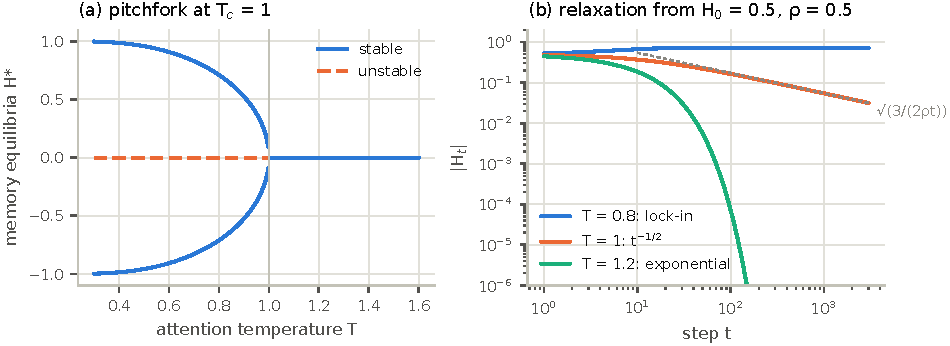
\includegraphics[width=\textwidth]{figures/fig_bifurcation.pdf}
\caption{Two-point attention memory, $\rho=0.5$. (a) Equilibria versus temperature: pitchfork at $T_c=1$. (b) Relaxation of $\lvert H_t\rvert$: lock-in at $T=0.8$, the algebraic law $(3/2\rho t)^{1/2}$ at $T=1$, exponential decay at $T=1.2$.}
\label{fig:bif}
\end{figure}

\begin{figure}[t]
\centering
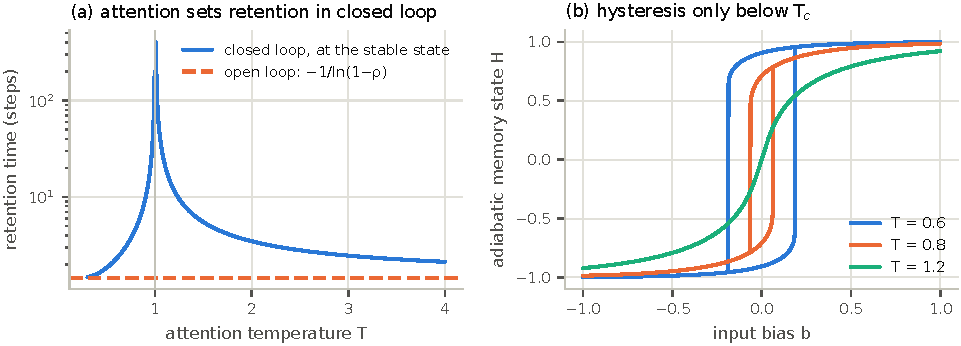
\includegraphics[width=\textwidth]{figures/fig_retention.pdf}
\caption{(a) Retention time at the stable equilibrium in closed loop (blue) against the open-loop value $-1/\ln(1-\rho)$ (orange): attention sets retention near $T_c$. (b) Adiabatic memory state under a slow sweep of the input bias: loops for $T<1$, a single-valued response at $T=1.2$.}
\label{fig:retention}
\end{figure}

\subsection{Multifractal module}\label{sec:cascade}
For multipliers driven by a two-state Markov chain, $\tau(q)=(q-1)D_q=-\log_2\rho(M_q)$ with $M_q(s,s')=\sum_cw_c(s)^qP(s'\mid s,c)$; the annealed partition function $\pi_0^{\mathsf T}M_q^n\mathbf1$ matches exact enumeration to $7\times10^{-16}$, and the i.i.d.\ limit returns the binomial value exactly (\V{V18}); for the reference chain $D_1=0.916$, $D_2=0.828$. For a continuous memory carried down the tree, $h'=(1-\rho)h\pm\rho$ with left share $\sigma((h+0.3)/0.8)$, the spectrum is the leading eigenvalue of a transfer operator: $\tau(2)=0.49709$ (converged in the grid), against enumeration slopes $0.50360$, $0.49916$, $0.49815$ for $n=10{\to}18$, $14{\to}20$, $16{\to}22$, converging toward it (\V{V19}). The binomial cascade with the same $D_1=0.8222$ ($p=0.7430$) has $D_2=0.694$; the memory cascade has $D_2=0.497$. Expectation E-A is met on both counts: memory changes the spectrum, and the change stays inside the thermodynamic formalism (\cref{fig:cascade}). A claim of novelty would need the attention parameterization to predict a measured spectrum from fewer parameters than a matched Markov cascade.

\begin{figure}[t]
\centering
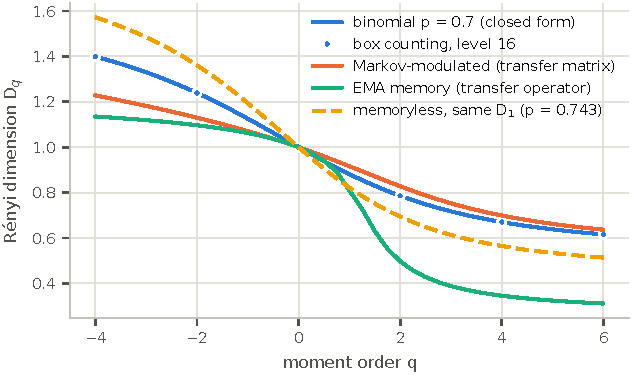
\includegraphics[width=0.7\textwidth]{figures/fig_cascades.pdf}
\caption{Rényi spectra. Binomial cascade (closed form and box counting), Markov-modulated cascade (transfer matrix), memory cascade (transfer operator), and the memoryless binomial with the memory cascade's $D_1$.}
\label{fig:cascade}
\end{figure}

\subsection{Wake module}\label{sec:wake}
For $W_{tt}+\gamma W_t-v^2\Delta W=f$ on a periodic grid with the $(2d+1)$-point Laplacian, the centered scheme
\[
(1+\tfrac{\gamma\Delta t}2)W^{n+1}=2W^n-(1-\tfrac{\gamma\Delta t}2)W^{n-1}+\Delta t^2\bigl(v^2\Delta_hW^n+f^n\bigr)
\]
is second order (observed $1.998$, \V{V34}) and stable for $v\Delta t/\Delta x<1/\sqrt d$ for every $\gamma\Delta t$ (Jury conditions, confirmed by bisection over the discrete spectrum to $6\times10^{-11}$, \V{V33}) \cite{Strikwerda2004}. With $E^{n+\frac12}=\tfrac12\lVert(W^{n+1}-W^n)/\Delta t\rVert^2+\tfrac{v^2}2\langle\nabla_hW^{n+1},\nabla_hW^n\rangle$ it satisfies the exact identity
\[
E^{n+\frac12}-E^{n-\frac12}=-\gamma\Delta t\Bigl\lVert\frac{W^{n+1}-W^{n-1}}{2\Delta t}\Bigr\rVert^2+\Delta t\Bigl\langle f^n,\frac{W^{n+1}-W^{n-1}}{2\Delta t}\Bigr\rangle,
\]
verified to $9\times10^{-15}$ in a forced, damped 2D run (\V{V35}); the solver records work and dissipation as observability hooks. The memory couples through \code{HybridWake}, the zero-order hold of F27.

\begin{figure}[t]
\centering
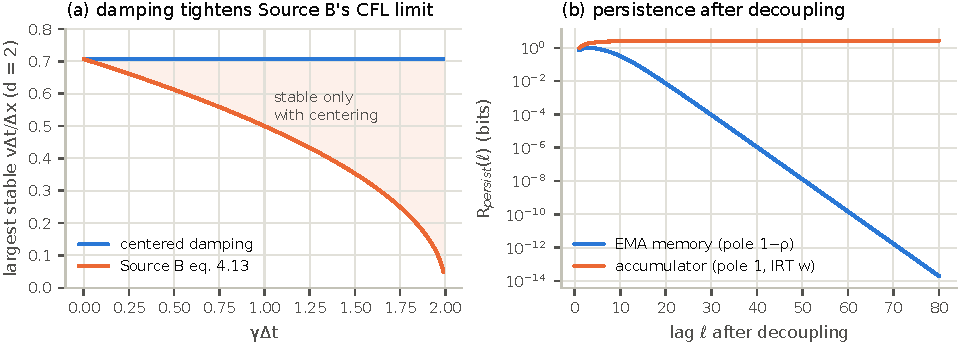
\includegraphics[width=\textwidth]{figures/fig_wake_persist.pdf}
\caption{(a) Largest stable Courant number in 2D for centered damping and for Source~B's eq.~(4.13). (b) $R_{\mathrm{persist}}(\ell)$ after decoupling for an EMA memory and an accumulator; under H1 it is identically zero (not drawable on a log scale).}
\label{fig:wake}
\end{figure}

%=====================================================================
\section{Revised claim ledger}
%=====================================================================

\begin{longtable}{@{}>{\raggedright\arraybackslash}p{0.75cm}>{\raggedright\arraybackslash}p{6.0cm}>{\raggedright\arraybackslash}p{4.2cm}>{\raggedright\arraybackslash}p{4.0cm}@{}}
\caption{Claims of Draft 1.0 after Phases 2--3.}\label{tab:ledger}\\
\toprule
& Claim (draft \S) & Classification & Note \\
\midrule\endfirsthead
\toprule & Claim (draft \S) & Classification & Note \\ \midrule\endhead
C1 & Four-equation system is a coherent state-space model (\S3, \S11) & construction, defective; repaired & F1--F5; \eqref{eq:core} \\
C2 & Softmax weights are a distribution (\S3.1) & theorem (trivial) & --- \\
C3 & E4 implements selective memory integration (\S3.1) & construction & content selection in open loop; retention also set by attention in closed loop (P2$'$) \\
C4 & A memory-dependent physical term may exist (\S3.2) & conjecture (H2), \lvl{2} & a stateful controller unless a new coupling is specified \\
C5 & $\mathcal L_{\mathrm{IWME}}$ is a language (\S4) & construction, incomplete & symbolic dynamics after F14 \\
C6 & $H_n=n\,h_2(p)$ (\S4.2) & theorem (standard) & \V{V17} \\
C7 & $D_1\approx0.8813$, $D_2\approx0.7859$ at $p=0.7$ & theorem (closed form) & \V{V15}; baseline \\
C8 & A recurring $D_q$ identifies related scaling (\S4.1) & weak conjecture & necessary condition only \\
C9 & Future expression depends on unrecoverable history (\S5) & trivial or unfalsifiable & F18, \cref{prop:P1} \\
C10 & Cross-environment invariant E12 (\S5) & conjecture & F21 \\
C11 & IRT $w$ as memory (\S5.1) & integrator; geometry recomputed & \cref{sec:irt}; F23 \\
C12 & Wake equation models information disturbances (\S6) & damped wave; physical identification unsupported & \cref{sec:sourceB,sec:wake} \\
C13 & Memory-coupled wake (\S6) & construction after F27 & \code{HybridWake} \\
C14 & H1/H2 distinction (\S7) & construction of hypotheses & retained as $C_E\equiv0$ versus $C_E\ne0$ \\
C15 & $R$ measures presence (\S7.2) & transfer entropy; ``presence'' \lvl{3} & replaced by $R_{\mathrm{persist}}$ \\
C16 & $\Delta_{\mathrm{IWME}}$ criterion (\S9) & construction & needs matched information access \\
C17 & The draft draws on Source D's attention measurements & unsupported & \cref{sec:sourceD} \\
C18 & Attention has a foundational operational role (\S1.1, \S7) & conjecture, sharpened & necessary for content selection, bistability and closed-loop retention; the persistence floor is set by $\rho$ \\
C19 & ``This closes the recursive cycle'' (\S7.1) & unsupported as written; repaired & F2 \\
C20 & ``Matter does not need to understand mathematics'' (\S11) & rhetorical, \lvl{3} & move to Discussion \\
\bottomrule
\end{longtable}
No claim of Draft~1.0 is empirically supported or independently replicated; this matches the draft's integrity note. Source claims found false or uninformative are listed in \cref{sec:sources} and Appendix~\ref{app:verify}.

%=====================================================================
\section{Interrogation of the draft's questions, revised}
%=====================================================================

\begin{enumerate}[label=\arabic*.]
\item \emph{Is nonuniform selection necessary for structured memory?} For the persistence floor set by $\rho$, no; for content selection, bistability and attention-dependent retention, yes (P2, P2$'$, P3).
\item \emph{Persistent memory with uniform attention?} Yes, with $\tau_{\mathrm{mem}}=-1/\ln(1-\rho)$; in closed loop sharp attention moves the retention time between $\tau_{\mathrm{mem}}$ and divergence at $T_c$ (aligned values) or shortens it (anti-aligned).
\item \emph{Retention improved or suppressed?} Both occur in closed loop, depending on the spectrum of the key--value cross-covariance (P3$'$).
\item \emph{Stable attractors from selective coupling?} Yes for $T<T_c$; none for $T>D_vD_k/4$ (\cref{lem:popoviciu}).
\item \emph{Entropy-rate change?} Memory changes the spectrum ($D_2$: $0.497$ against $0.694$ at matched $D_1$) through a transfer operator.
\item \emph{Cross-scale preservation?} The memory cascade has a well-defined spectrum in the limit; finite-$n$ corrections decay like $1/n$.
\item \emph{History-dependent geometry?} Only through $C_E\ne0$ (H2) or representation (H1); $R_{\mathrm{persist}}$ measures it after decoupling.
\item \emph{Disappears under ablation?} Bistability, hysteresis and the attention-dependent excess retention, yes; the $\rho$-floor, no.
\item \emph{Equivalent outcomes from conventional filters?} Persistence, yes (the EMA is an IIR filter). Bistability and hysteresis require a nonlinear unit, and any saturating recurrent unit with loop gain above one produces both.
\item \emph{Non-anthropomorphic physical attention?} Gibbs weighting of competing modes with saturation (F12).
\end{enumerate}
\emph{The investigator's closing question}, whether attention is needed for the dynamics or only for observing them, has a precise form: it is the question $C_E\equiv0$ or $C_E\ne0$, which no observational statistic settles (\cref{prop:P1}) and which Protocol~B and interventions on the memory substrate can test.

%=====================================================================
\section{Engineering: the kgirl integration}
%=====================================================================

The package \code{src/kgirl/iwme} follows the conventions of \code{kgirl.nihiline}: numpy-only modules with optional sympy, a command-line interface, unittest suites, and figures generated from code.
\begin{center}\small
\begin{tabularx}{\textwidth}{@{}l>{\raggedright\arraybackslash}X@{}}
\toprule
Module & Content \\
\midrule
\code{attention} & P2, P2$'$, \cref{lem:popoviciu}, P3, P3$'$, hysteresis, gated forgetting \\
\code{cascade} & binomial, Markov and memory cascades; transfer operator; Hutchinson fixed point \\
\code{irt} & IRT metric, determinant, rank, singular circles, curvature (three routes), Source~C transcriptions \\
\code{wake} & centered and Source~B schemes, CFL and order, energy identity, zero-order hold, Source~B checks \\
\code{sources} & Source~D Tier 1--2 checks, coherence measures \\
\code{core} & repaired core \eqref{eq:core}, exact $R_{\mathrm{persist}}$ \\
\code{verify} & the 47-check registry; table, JSON and \LaTeX{} output (Appendix~\ref{app:verify}) \\
\code{plots} & the five figures of this report \\
\bottomrule
\end{tabularx}
\end{center}
The harness MCP server gains three tools: \code{iwme\_verify}, \code{iwme\_irt\_point} and \code{iwme\_attention}. Before editing \code{harness/mcp\_server.py}, its blast radius was computed with the repository's Atlas index: five dependents, all inside kgirl (two test modules, the CLI and its entry point, the nihiline tests); the harness, nihiline and evolve suites pass after the change. The 70 IWME unit tests pass in about 15\,s. Branch \code{claude/iwme-phase3} holds the work; merging is left to the investigator.

%=====================================================================
\section{Checkpoint and next actions}
%=====================================================================

\begin{itemize}
\item[Q1] Definition of ``intra-dimensional'' and ``emission'': open (candidate readings in F6 and \cref{sec:core}).
\item[Q2] Sources B, C, D: supplied and audited; Source E received and outside scope.
\item[Q3] Narrowing to the inductive-bias claim with $C_E\ne0$ as extension M4: clarification received (\cref{sec:hypothesis}); a formal decision is still requested.
\item[Q4] Execution environment: used; every number in this report is computed.
\item[Q5] Physical data or apparatus for Experiments B, C, F: open. Phase~4 proceeds simulation-first.
\item[Q6] Authorship and venue: open.
\end{itemize}
\paragraph{Phase 4.} (A) multifractal experiment with pre-registered symbolization and parameter-count-matched model comparison; (B) Protocol B on a nonlinear simulated plant, then on a physical pattern-forming system if Q5 allows; (E) attention ablation in a mode-competition system (Swift--Hohenberg with Gibbs mode weighting, F12), sweeping $T$ through $T_c$ and measuring hysteresis at extrapolated sweep rate; (F) wake perturbation with the zero-order-hold source and pre-registered $P_E$.

%=====================================================================
\section{Adversarial reviewer's verdict}
%=====================================================================

Draft~1.0 remains unready for submission: its core, as written, conflates observation with actuation and leaves the loop open, and its presence criterion measures coupling. The repaired core of \cref{sec:core} is coherent, and the attention mechanism now carries precise, falsifiable predictions: a pitchfork at $T_c$, algebraic slowing with exponent $\tfrac12$, hysteresis area scaling as $(1-T)^2$, and flip or Neimark--Sacker crossings set by the key--value geometry. The supplied sources must enter with care. Source~C's IRT is a well-defined manifold with a nondegenerate metric off ten located circles, and its published metric, Christoffel symbols, curvature and shadow integral are wrong. Source~B's categorical statements are ill-typed and its wake system has six identified defects; its finite fixed-point content survives as the Hutchinson model. Source~D supplies no usable measurement. The strongest recoverable material is the H1/H2 axis, the attention bifurcation, the identifiability statement, and an exact persistence criterion that tells the program where evidence can come from.

\paragraph{Evidence and speculation.} Established (\lvl{0}): every proposition, lemma and numerical check above. Extrapolation (\lvl{1}): that the gated and memory-cascade variants describe classes of physical systems. Hypothesis (\lvl{2}): the parametric IWME claim of \cref{sec:hypothesis} and M4. Speculative (\lvl{3}): presence as more than state incompleteness; any reading of the IRT as a communication device.

%=====================================================================
\appendix
\section{Verification registry}\label{app:verify}
%=====================================================================
Generated from the repository root by
\begin{flushleft}\small\code{PYTHONPATH=src python -m kgirl.iwme verify -{}-latex research/iwme/verification\_table.tex}\end{flushleft}
``Observed'' is the program's output. A refutation of a source claim appears as a passing check. All 47 checks pass.

{\footnotesize
\begin{longtable}{@{}p{0.75cm}p{0.35cm}>{\raggedright\arraybackslash}p{6.6cm}>{\raggedright\arraybackslash}p{6.2cm}p{0.9cm}@{}}
\toprule
Id & L & Claim & Observed & Result \\
\midrule\endfirsthead
\toprule Id & L & Claim & Observed & Result \\ \midrule\endhead
\verifyrows
\bottomrule
\end{longtable}
}

\section{Notation}\label{app:notation}
$X_t$ physical state; $H_t$ memory; $A_t$ attention weights; $Y_t$ interaction signal; $E_t$ environment parameters; $U_t$ controls; $C_E$ actuation map; $\Pi_{E,\lambda}$ perspective map; $T$ attention temperature; $\rho$ write rate; $\gamma$ wake damping (Source~B's $\lambda$); $\lambda$ observational scale; $\mathrm H[\cdot]$ entropy. IRT: $u=R-r\cos\varphi$, $\rho=ue^{-\alpha\psi}$ (radius of the $\theta$-circle; the memory write rate $\rho$ never appears in the IRT sections), $D=\beta r\sin^2\varphi\cosh\beta\psi+\alpha u\cos\varphi\sinh\beta\psi$.

\clearpage\phantomsection\addcontentsline{toc}{section}{References}
\begin{thebibliography}{99}\footnotesize\setlength{\itemsep}{1pt plus 0.5pt}\setlength{\parskip}{0pt}
\bibitem{SourceA} K1ll. \emph{Intra-dimensional Working Memory Emission}, Draft 1.0. Unpublished manuscript.
\bibitem{SourceB} Anonymous. \emph{The Emergent Fractal Law and the $3^{627}$ Framework: A Categorical Theory of Self-Similar Information Geometry}. Unpublished manuscript, 21 October 2025.
\bibitem{SourceC} Neurotronic Phase Caster Research Collective. \emph{Geometry as Emergent Uni-telligence: The Informational Handshake of Higher-Dimensional Coherence Measurement}. Unpublished manuscript, 7 November 2025.
\bibitem{SourceD} J.\ Edwards (with D.\ J.\ McConnell). \emph{The Convergence Point: A Developmental Framework for Machine Consciousness}. Manuscript.
\bibitem{SourceE} M.\ Oo et al. \emph{From Triangle to Form: Bridging Discrete Relational Networks to Continuum Spacetime and Hadronic Droplets via E8 Holographic Hydrodynamics}. Manuscript, 2026.
\bibitem{Shannon1948} C.\ E.\ Shannon. A mathematical theory of communication. \emph{Bell Syst.\ Tech.\ J.} 27:379--423, 623--656, 1948.
\bibitem{ConantAshby1970} R.\ C.\ Conant, W.\ R.\ Ashby. Every good regulator of a system must be a model of that system. \emph{Int.\ J.\ Syst.\ Sci.} 1(2):89--97, 1970.
\bibitem{Mandelbrot1974} B.\ B.\ Mandelbrot. Intermittent turbulence in self-similar cascades. \emph{J.\ Fluid Mech.} 62:331--358, 1974.
\bibitem{Hentschel1983} H.\ G.\ E.\ Hentschel, I.\ Procaccia. The infinite number of generalized dimensions of fractals and strange attractors. \emph{Physica D} 8:435--444, 1983.
\bibitem{Halsey1986} T.\ C.\ Halsey, M.\ H.\ Jensen, L.\ P.\ Kadanoff, I.\ Procaccia, B.\ I.\ Shraiman. Fractal measures and their singularities. \emph{Phys.\ Rev.\ A} 33:1141--1151, 1986.
\bibitem{Renyi1961} A.\ Rényi. On measures of entropy and information. \emph{Proc.\ 4th Berkeley Symp.} 1:547--561, 1961.
\bibitem{Ruelle1978} D.\ Ruelle. \emph{Thermodynamic Formalism}. Addison-Wesley, 1978.
\bibitem{LindMarcus1995} D.\ Lind, B.\ Marcus. \emph{An Introduction to Symbolic Dynamics and Coding}. Cambridge University Press, 1995.
\bibitem{Hutchinson1981} J.\ E.\ Hutchinson. Fractals and self-similarity. \emph{Indiana Univ.\ Math.\ J.} 30:713--747, 1981.
\bibitem{Takens1981} F.\ Takens. Detecting strange attractors in turbulence. \emph{Lecture Notes in Math.} 898:366--381, 1981.
\bibitem{Kalman1960} R.\ E.\ Kalman. A new approach to linear filtering and prediction problems. \emph{J.\ Basic Eng.} 82:35--45, 1960.
\bibitem{Granger1969} C.\ W.\ J.\ Granger. Investigating causal relations by econometric models and cross-spectral methods. \emph{Econometrica} 37:424--438, 1969.
\bibitem{Schreiber2000} T.\ Schreiber. Measuring information transfer. \emph{Phys.\ Rev.\ Lett.} 85:461--464, 2000.
\bibitem{Pearl2009} J.\ Pearl. \emph{Causality}, 2nd ed. Cambridge University Press, 2009.
\bibitem{Rissanen1978} J.\ Rissanen. Modeling by shortest data description. \emph{Automatica} 14:465--471, 1978.
\bibitem{Bahdanau2015} D.\ Bahdanau, K.\ Cho, Y.\ Bengio. Neural machine translation by jointly learning to align and translate. \emph{ICLR}, 2015.
\bibitem{Vaswani2017} A.\ Vaswani et al. Attention is all you need. \emph{NeurIPS} 30, 2017.
\bibitem{Gers2000} F.\ A.\ Gers, J.\ Schmidhuber, F.\ Cummins. Learning to forget: continual prediction with LSTM. \emph{Neural Comput.} 12:2451--2471, 2000.
\bibitem{Hopfield1982} J.\ J.\ Hopfield. Neural networks and physical systems with emergent collective computational abilities. \emph{PNAS} 79:2554--2558, 1982.
\bibitem{Kuznetsov2004} Yu.\ A.\ Kuznetsov. \emph{Elements of Applied Bifurcation Theory}, 3rd ed. Springer, 2004.
\bibitem{Kuramoto1984} Y.\ Kuramoto. \emph{Chemical Oscillations, Waves, and Turbulence}. Springer, 1984.
\bibitem{Turing1952} A.\ M.\ Turing. The chemical basis of morphogenesis. \emph{Phil.\ Trans.\ R.\ Soc.\ B} 237:37--72, 1952.
\bibitem{CrossHohenberg1993} M.\ C.\ Cross, P.\ C.\ Hohenberg. Pattern formation outside of equilibrium. \emph{Rev.\ Mod.\ Phys.} 65:851--1112, 1993.
\bibitem{Mermin1979} N.\ D.\ Mermin. The topological theory of defects in ordered media. \emph{Rev.\ Mod.\ Phys.} 51:591--648, 1979.
\bibitem{Strikwerda2004} J.\ C.\ Strikwerda. \emph{Finite Difference Schemes and Partial Differential Equations}, 2nd ed. SIAM, 2004.
\bibitem{ONeill1983} B.\ O'Neill. \emph{Semi-Riemannian Geometry with Applications to Relativity}. Academic Press, 1983.
\bibitem{doCarmo1992} M.\ P.\ do Carmo. \emph{Riemannian Geometry}. Birkhäuser, 1992.
\bibitem{DGMS1975} P.\ Deligne, P.\ Griffiths, J.\ Morgan, D.\ Sullivan. Real homotopy theory of Kähler manifolds. \emph{Invent.\ Math.} 29:245--274, 1975.
\bibitem{Walsh1923} J.\ L.\ Walsh. A closed set of normal orthogonal functions. \emph{Amer.\ J.\ Math.} 45:5--24, 1923.
\end{thebibliography}
\noindent{\footnotesize Classical references are given from standard bibliographic records; page ranges should be checked against the publishers' records before submission.}

\end{document}
